\section{Piecewise Quadratic Model}

In this section, we will examine the dynamics of a piecewise quadratic model.
Starting with a model with 4 branches and symmetry, like in \Cref{sec:og.full}.
After that, we will reduce the model to just two branches using symmetry.

\subsection{Full Model}

The full model is the map $x \mapsto f(x) \mod 6$.
Where $f$ is given by the following collection of equations.
\begin{align}
    f(x) & = \begin{cases}
        g(x) & \text{if } r(x) < 3 \\
        g(x) + 3 & \text{else}
    \end{cases} \label{equ:quad.full.f} \\
    g(x) & = \begin{cases}
        a_L \cdot s_L(x)^2 + b_L \cdot x + c_L & \text{if } s(x) < \frac{3}{2} \\
        a_R \cdot s_R(x)^2 + b_R \cdot x + c_R & \text{else}
    \end{cases} \label{equ:quad.full.g}
\end{align}

\Cref{equ:quad.full.f} causes the disontinuity in the middle at $x = 3$.
It also makes sure, the symmetry $f(x + 3) \equiv f(x) + 3 \mod 6$ is true.
Each half of the model is then governed by \Cref{equ:quad.full.g}.
Here all the 6 parameters $a_L, a_R, b_L, b_R, c_L,$ and $c_R$ act.

\Crefrange{equ:quad.full.s}{equ:quad.full.sr} provide adjusted values of x for either choosing between branches in both halves or substituting in the quadratic formulas of each branch.
\begin{subequations}
\begin{align}
    s(x) & = x \mod 3 \label{equ:quad.full.s} \\
    s_L(x) & = s(x) - \frac{3}{4} \\
    s_R(x) & = s(x) - \frac{9}{4} \label{equ:quad.full.sr}
\end{align}
\end{subequations}

\Cref{fig:quadratic.full.2d.full} shows a 2D-scan of the periods of the stable cycles.
The parameters $a_L = a_R = 1$ and $b_L = b_R = 0$ are fixed and the parameters $c_L$ and $c_R$ are varied.
Both are varied within the range $[0, 6]$ because beyond that the diagram just repeats infinitely.
The structure in the bottom left corner is enhanced and depicted in \Cref{fig:quadratic.full.2d.z1}.
\begin{figure}
    \centering
    \begin{subfigure}{0.4\textwidth}
        \centering
        \includegraphics[width=\textwidth]{21_Quadratic_mod6/2D_Period_Full/result.png}
        \caption{Full}
        \label{fig:quadratic.full.2d.full}
    \end{subfigure}
    \begin{subfigure}{0.4\textwidth}
        \centering
        \includegraphics[width=\textwidth]{21_Quadratic_mod6/2D_Period_Zoomed1/result.png}
        \caption{Zoomed}
        \label{fig:quadratic.full.2d.z1}
    \end{subfigure}
    \caption{2D Scan of Full Quadratic Model}
\end{figure}
